\documentclass[11pt]{article}
\usepackage[a4paper,margin=2.3cm]{geometry}
\ifdefined\XeTeXrevision\else\usepackage[T1]{fontenc}\fi
\usepackage{amsmath,amssymb}
\usepackage{newtxtext,newtxmath}
\ifdefined\XeTeXtracingfonts\XeTeXtracingfonts=0\fi
\usepackage{graphicx}
\usepackage{booktabs}
\usepackage{array}
\usepackage[font=small,labelfont=bf,labelsep=period,justification=justified,singlelinecheck=false]{caption}
\usepackage{setspace}
% lineno.sty contains a Latin-1 byte; read it as Latin-1 under XeTeX (tectonic) to avoid an encoding warning
\ifdefined\XeTeXrevision\XeTeXdefaultencoding "iso-8859-1"\fi
\usepackage[switch,pagewise]{lineno}
\ifdefined\XeTeXrevision\XeTeXdefaultencoding "utf-8"\fi
\usepackage[hidelinks]{hyperref}
\usepackage{url}
% allow line breaks after hyphens in long URLs
\Urlmuskip=0mu plus 1mu
\expandafter\def\expandafter\UrlBreaks\expandafter{\UrlBreaks\do\-}
\usepackage[super,comma,sort&compress]{natbib}
\setcitestyle{super}
\setlength{\parskip}{3pt}
\setlength{\emergencystretch}{2em}

\newcommand{\Tr}{\operatorname{Tr}}
\newcommand{\tr}{\operatorname{tr}}
\newcommand{\C}{\mathbb{C}}
\newcommand{\R}{\mathbb{R}}
\newcommand{\Z}{\mathbb{Z}}
\newcommand{\one}{\mathbf{1}}
\newcommand{\IME}{I_{\mathrm{ME}}}
\newcommand{\FD}{F_{\mathrm{DKZ}}}
\newcommand{\Li}{\operatorname{Li}_2}
\newcommand{\Cl}{\operatorname{Cl}_2}
\renewcommand{\Re}{\operatorname{Re}}
\renewcommand{\Im}{\operatorname{Im}}

\begin{document}
\onehalfspacing

\begin{center}
{\LARGE\bfseries Fourier measurements are optimal for CGLMP Bell tests\\[2pt] on maximally entangled states in every dimension\par}
\vspace{10pt}
{\large Ansh Mishra$^{1,\ast}$ and Aryan Senthilkumar$^{2}$\par}
\vspace{6pt}
{\small $^{1}$Independent researcher, Cumming, GA, USA\par
$^{2}$Independent researcher, Johns Creek, GA, USA\par
E-mail: \href{mailto:ansh.mishra2025@gmail.com}{ansh.mishra2025@gmail.com} (A.M.),
\href{mailto:aryan.senthilk@gmail.com}{aryan.senthilk@gmail.com} (A.S.)\par
$^\ast$Corresponding author\par}
\end{center}

\linenumbers

\begin{abstract}
\noindent Bell inequalities certify that correlations between distant measurements have no local explanation, and in
high dimensions they underpin device-independent tests of entanglement and randomness. The
Collins--Gisin--Linden--Massar--Popescu (CGLMP) inequalities are the standard Bell inequalities for two parties with
$d$ outcomes per measurement. On the maximally entangled state of two $d$-level systems the largest known violation
is produced by Fourier-type measurements found by Durt, Kaszlikowski and \.Zukowski (DKZ). Whether other measurements
can do better was posed as part of Open Quantum Problem~27 of IQOQI Vienna. Here we prove that, for every number of
outcomes $d$ and for maximally entangled states of any local dimension, no projective measurements exceed the DKZ
value, and that the DKZ measurements are the only optimal ones up to local unitaries and an inert auxiliary system.
The key new ingredient is a matrix inequality on a strip in the complex plane, which we prove for matrices of every
size by exhibiting an explicit positive density in a two-variable extension of Stahl's theorem, formerly the
Bessis--Moussa--Villani conjecture. A computer-assisted certificate, checked in interval arithmetic, connects this
inequality to the Bell problem for every $d$. For $d\le20$ the entire proof, including this certificate, is checked
by the Lean theorem prover. Together with earlier work on Part~A and our results on the two remaining clauses of
Part~B, this completes the resolution of Problem~27 as originally posed; the verdict on its noise-resistance clause
depends on how noise resistance is measured.
\end{abstract}

%==============================================================================================================
\noindent Bell's theorem states that the correlations between measurements on distant quantum systems can be stronger
than any local hidden-variable model allows\cite{Bell1964,CHSH1969,Brunner2014}. Loophole-free experiments have
confirmed such violations\cite{Hensen2015,Giustina2015,Shalm2015}, and a violation can certify, without trusting the
devices, that entanglement is present, that outcomes are random or that a key is secret\cite{Acin2007,Pironio2010}.
Each of these applications rests on a quantitative fact: for a given Bell expression one must know the largest value
that quantum mechanics allows, and which states and measurements attain it. For two parties with two settings and two
outcomes this is Tsirelson's bound\cite{Tsirelson1980} for the Clauser--Horne--Shimony--Holt inequality\cite{CHSH1969}.

High-dimensional entanglement is now produced routinely in photonic platforms\cite{Erhard2020,Dada2011}, and Bell tests
with many outcomes can tolerate more noise and lower detection efficiencies than tests with qubits\cite{KGZMZ2000,
CGLMP2002,Vertesi2010}. The canonical Bell inequalities for this setting were found by Collins, Gisin, Linden, Massar
and Popescu (CGLMP)\cite{CGLMP2002}, with an equivalent form for $d=3$ by Kaszlikowski and co-workers\cite{KKCZO2002}.
For the maximally entangled state of two $d$-level systems, the measurements found numerically by Kaszlikowski
\textit{et al.}\cite{KGZMZ2000} and described analytically by Durt, Kaszlikowski and \.Zukowski (DKZ)\cite{DKZ2001},
namely phase shifts followed by a discrete Fourier transform, give the largest known CGLMP value. Numerical searches
never found anything better\cite{KGZMZ2000,DKZ2001,CGLMP2002}. Whether the DKZ measurements are necessarily the optimal
ones was asked by Gill\cite{Gill2007} and is Part~B of Open Quantum Problem~27 of IQOQI Vienna\cite{OQP27}, a list of
problems that goes back to ref.~\citenum{KruegerWerner2005}.

Here we answer the maximally entangled part of that question for every number of outcomes $d$. No projective
measurements on a maximally entangled state of any local dimension exceed the DKZ value, and the DKZ measurements are
the only optimal ones up to local unitaries and an inert auxiliary system. The proof combines an exact reduction to a
long-range clock model, a new inequality for non-normal matrices whose real part is a projection, and a
computer-assisted certificate for a discrete step. The matrix inequality is the heart of the argument. We prove it for
matrices of every size by uncovering an explicit positive density behind a two-variable extension of the Laplace
representation of Bessis, Moussa and Villani (BMV), which was conjectured in 1975 and proved by Stahl\cite{BMV1975,
Stahl2013}. The argument has also been formalised in the Lean theorem prover\cite{Lean2021,Mathlib2020}. The formal
proof is complete except for one input, the certificate for $d\ge21$. For $d\le20$ Lean checks the certificate
as well, so for these $d$ the result is fully machine-checked. The matrix inequality and the positivity theorem behind
it are formalised in full, for matrices of every size. We also settle the two remaining clauses of Part~B, on noise
resistance and on Kullback--Leibler discrimination (Table~\ref{tab:status}).

%==============================================================================================================
\section*{The CGLMP inequality and the question}

Alice and Bob each choose one of two settings, $x,y\in\{1,2\}$, and obtain outcomes $A_x,B_y\in\Z_d=\{0,\dots,d-1\}$
(Fig.~\ref{fig:1}a). The CGLMP expression is\cite{CGLMP2002}
\begin{multline}\label{eq:cglmp}
I_d=\sum_{k=0}^{\lfloor d/2\rfloor-1}\Bigl(1-\frac{2k}{d-1}\Bigr)\Bigl(\bigl[P(A_1=B_1+k)+P(B_1=A_2+k+1)
+P(A_2=B_2+k)+P(B_2=A_1+k)\bigr]\\
-\bigl[P(A_1=B_1-k-1)+P(B_1=A_2-k)+P(A_2=B_2-k-1)+P(B_2=A_1-k-1)\bigr]\Bigr),
\end{multline}
where $P(A_x=B_y+k)$ is the probability that $A_x-B_y\equiv k\pmod d$. The four pairs of settings form a chain
$A_1,B_1,A_2,B_2,A_1$. The expression rewards outcomes that are close on the $d$-hour clock in one direction
along the chain and penalizes the other direction, and the extra shift by one in the term $P(B_1=A_2+k+1)$ makes it
impossible for a local model to be perfectly correlated all around the chain. Local hidden-variable models obey
$I_d\le2$\cite{CGLMP2002}. For $d=2$ the expression reduces to the Clauser--Horne--Shimony--Holt expression.

We consider the maximally entangled state $|\Phi_D\rangle=D^{-1/2}\sum_{j=1}^{D}|j\rangle|j\rangle$ of two systems
of an arbitrary dimension $D$, and projective measurements $\{P^x_a\}_{a\in\Z_d}$ for Alice and $\{Q^y_b\}_{b\in\Z_d}$
for Bob, so that $P(A_x=a,B_y=b)=\langle\Phi_D|P^x_a\otimes Q^y_b|\Phi_D\rangle$. The DKZ measurements act on
$D=d$: each party applies the phases $e^{2\pi ij\theta/d}$ to the basis states $|j\rangle$, with $\theta=0,\frac12$ for
Alice's two settings and $\theta=\frac14,-\frac14$ for Bob's, then a discrete Fourier transform, and measures in the
computational basis. They give\cite{DKZ2001,CGLMP2002}
\begin{equation}\label{eq:IME}
\IME(d)=\frac{4}{d(d-1)}\sum_{j=1}^{d-1}(d-j)\sec\frac{\pi j}{2d},
\end{equation}
for example $\IME(2)=2\sqrt2$, $\IME(3)=2.8729\ldots$ and $\IME(10)=2.9398\ldots$. As $d\to\infty$, $\IME(d)$
tends to $32G/\pi^2=2.9698\ldots$, where $G$ is Catalan's constant (Fig.~\ref{fig:1}c).

Two features make this problem natural and hard. First, it is a statement about the maximally entangled state, the
natural target state of high-dimensional sources and the state for which the DKZ measurements were designed. It is not
the same as
the maximal CGLMP value over all states: for $d\ge3$ that maximum is attained by states that are not maximally
entangled\cite{ADGL2002,MethotScarani2007,ZohrenGill2008}, and it has been determined exactly only for small $d$
(refs~\citenum{IoannouRosset2021,repoCGLMP}). Second, the measurement operators of the two settings do not commute and
may act on a space of any dimension. A numerical search can only explore finitely many dimensions, and the
semidefinite hierarchies that bound quantum correlations\cite{NPA2008} certify one value of $d$ at a time.

Before this work the evidence was as follows. For $d=2$ the statement is Tsirelson's bound. For $d=3$ a semidefinite
relaxation agrees with the DKZ value to within $10^{-10}$ (ref.~\citenum{LVN2014}); this is the partial result listed
in ref.~\citenum{OQP27}. In earlier work we obtained exact sum-of-squares certificates, with cyclotomic coefficients,
proving optimality and rigidity of DKZ among projective measurements for $3\le d\le20$\cite{repoCGLMP}, and we proved
the statement for every $d$ in the special case in which the four link operators of the strategy coincide, which makes
the problem commutative\cite{classical2026}. Within a family of Fourier measurements with linear phase offsets, the
DKZ point was recently found numerically to be a strict local maximum for $d\le6$\cite{TMMD2026}. The certificates grow
quickly with $d$ and show no pattern that could be extrapolated, and relaxations that only use correlations among a
bounded number of settings fail for large $d$, even in the commutative case\cite{classical2026}.

\begin{figure}[t]
\centering
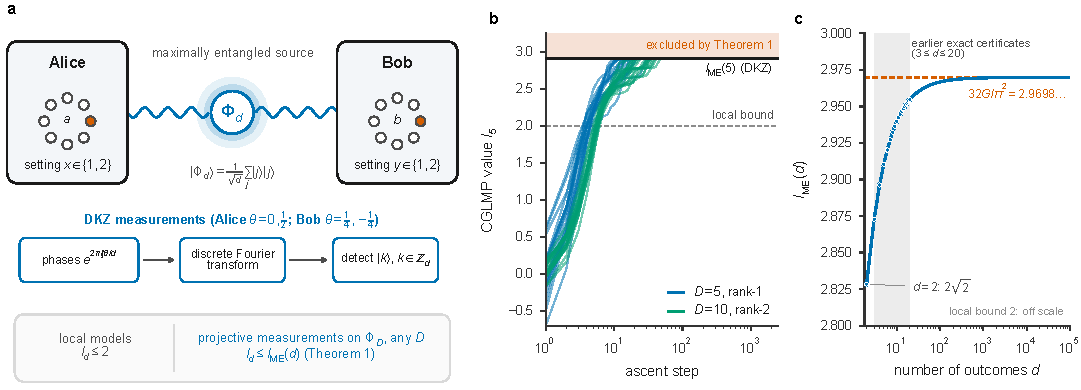
\includegraphics[width=\textwidth]{figures/fig1.pdf}
\caption{\textbf{The CGLMP Bell test on maximally entangled states.} \textbf{a}, A source distributes the maximally
entangled state $\Phi_d$. Alice and Bob each choose one of two settings and record one of $d$ outcomes; the CGLMP value
$I_d$ (equation~\eqref{eq:cglmp}) rewards outcomes that are close on the $d$-hour clock. The DKZ measurements apply
setting-dependent phases, a discrete Fourier transform and a computational-basis measurement. Local models obey
$I_d\le2$; Theorem~1 shows that every projective measurement on a maximally entangled state of any dimension obeys
$I_d\le\IME(d)$. \textbf{b}, Gradient ascent of $I_5$ over projective strategies on $\Phi_D$ from 40 random starting
points, 20 for each $D$ ($D=5$, rank-one projectors, blue; $D=10$, rank-two projectors, green). All runs stop at the DKZ value
$\IME(5)=2.9105\ldots$ (black line); the largest final value exceeds it by $4\times10^{-13}$, the floating-point
accuracy. The shaded region above $\IME(5)$ is excluded by Theorem~1. \textbf{c}, $\IME(d)$ for $2\le d\le10^5$. It
approaches $32G/\pi^2$ (dashed) from below, as $32G/\pi^2-0.3034/d$ for large $d$; dots mark $d\le20$, and the grey
band the range $3\le d\le20$ covered by our earlier exact certificates\cite{repoCGLMP}.}
\label{fig:1}
\end{figure}

%==============================================================================================================
\section*{Optimality and rigidity in every dimension}

Our main results are the following.

\medskip
\noindent\textbf{Theorem 1 (optimality).} \emph{For every $d\ge2$, every $D\ge1$ and all projective measurements of
Alice and Bob on $\C^D\otimes\C^D$, the CGLMP value of the maximally entangled state $\Phi_D$ satisfies
$I_d\le\IME(d)$. The DKZ measurements attain this value.}

\medskip
\noindent\textbf{Theorem 2 (rigidity).} \emph{If projective measurements on $\Phi_D$ attain $I_d=\IME(d)$, then $d$
divides $D$, and there is a unitary $u:\C^D\to\C^d\otimes\C^{D/d}$ such that the local unitary $u\otimes\bar u$ maps
the measurements to the DKZ measurements tensored with the identity on $\C^{D/d}$, and maps $\Phi_D$ to
$\Phi_d\otimes\Phi_{D/d}$. The unitary $u$ is unique up to $u\mapsto(\one_d\otimes u')u$. In particular, if $d$ does
not divide $D$, the maximal CGLMP value on $\Phi_D$ is strictly smaller than $\IME(d)$.}
\medskip

\noindent Theorem~1 identifies the largest CGLMP value of maximally entangled states for every $d$: it is the
Tsirelson-type bound of the CGLMP expression restricted to these states. Theorem~2 says that this value is attained in
an essentially unique way. Observing $I_d=\IME(d)$ with projective measurements on a maximally entangled state certifies
the measurements up to a local change of basis and an inert auxiliary system. This is a self-testing
statement\cite{MayersYao2004,SupicBowles2020} for measurements on maximally entangled states. It is weaker than full
device-independent self-testing, which would also have to certify the state. Device-independent self-tests of
maximally entangled states of every dimension are known for other Bell expressions, which are tailored to these
states\cite{SATWAP2017,Kaniewski2019,SSKA2021}; they do not determine the maximal value of $I_d$. Theorem~1 also gives a
dimension-free test. Within projective measurements, a value $I_d>\IME(d)$ rules out a maximally entangled source of
any local dimension.

Figure~\ref{fig:1}b illustrates the content of Theorem~1 for $d=5$. Gradient ascent over strategies started from random
measurements climbs from values near zero, crosses the local bound and stops at the DKZ value in every run, for rank-one
and rank-two projectors alike. Such numerics explore only finitely many dimensions and starting points, and they find
local maxima at best. Theorems~1 and~2 hold for every $d$ and every $D$.

The proofs of Theorems~3 and~4 below, which carry the new mathematics, are analytic. The proofs of Theorems~1 and~2 in
addition use a rigorous computer-assisted certificate for a family of inequalities between explicit kernels (CONE$_d$,
below). It is verified in interval arithmetic for every $d$: by explicit certificates for $d\le2000$ and by a proof with
certified error bounds for $d\ge2001$. All other steps are also verified in Lean, and so is CONE$_d$ for $d\le20$
(Methods). Theorems~1 and~2 are therefore proved for every $d$, with a computer-assisted step in interval arithmetic
for $d\ge21$, and fully formalised for $d\le20$; Theorems~3 and~4 are formalised in full. The statements concern
projective measurements; general positive-operator-valued measurements are not covered (Methods).

%==============================================================================================================
\section*{From Bell strategies to a clock model}

The first step is an exact reformulation\cite{classical2026}. Write $w=e^{2\pi i/d}$ and encode Alice's measurements
by the unitaries $U_x=\sum_aw^aP^x_a$ and Bob's by $U'_y=\sum_bw^bQ^y_b$. The CGLMP expression is invariant under a
cyclic group of order $4d$ that shifts the outcomes and rotates the chain of settings. Averaging over this group and
applying the Stone--von Neumann theorem for $\Z_d$ (Methods), every strategy on $\Phi_D$ becomes a family of $d$
unitaries $V_0,\dots,V_{d-1}$ on an auxiliary space, each of order four ($V_k^4=\one$), with
\begin{equation}\label{eq:clock}
I_d=\frac{4F(V)}{d(d-1)},\qquad F(V)=\sum_{0\le j<k\le d-1}\Re\bigl[h_{k-j}\,\tr(V_jV_k^\dagger)\bigr],\qquad
h_m=\sec\frac{\pi m}{2d}-i\csc\frac{\pi m}{2d},
\end{equation}
where $\tr$ is the normalized trace. Conversely every such family comes from a strategy. The DKZ strategy corresponds
to $V_0=\dots=V_{d-1}=\one$, so Theorem~1 is equivalent to $F(V)\le\FD:=\sum_{m=1}^{d-1}(d-m)\sec\frac{\pi m}{2d}$.

Equation~\eqref{eq:clock} describes a long-range clock model: $d$ sites carry four-state ``spins'' $V_k$, and every pair
of sites is coupled, with a complex coupling $h_{k-j}$ that depends on their distance. If the $V_k$ commute they can be
diagonalized together, and the model becomes a classical spin model. Its ground state is a single domain wall, which
we showed for every $d$ in ref.~\citenum{classical2026}. The quantum problem asks whether matrix-valued spins can
do better than classical ones. They cannot, but the argument has to deal with genuinely non-commuting configurations:
numerically, the reduced model has non-commuting local maxima that are not global maxima, and the classical proof does
not transfer.

A second reformulation explains where the difficulty sits. Collect the spectral projections of all $V_k$ into $4d$
projections $Q_x$ placed at the points $x$ of a circle with $4d$ sites (Methods). The function $F$ then becomes a
pairing of the projections at $x$ with those at $x+d$ through the kernel $\cot(\pi(x-y)/4d)$, which is the
kernel of the discrete Hilbert transform. In a continuum limit, in which the circle becomes continuous and the
projections become operator-valued functions, the classical theory is a theorem of Stein and Weiss: the distribution
of the conjugate function of an indicator function depends only on the measure of the set\cite{SteinWeiss1959}. This
theorem determines the continuum optimum, and the discrete problem differs from it by terms at the junctions between
blocks of the configuration. For commuting spins these two parts can be handled separately\cite{classical2026}. For
matrices, neither the continuum statement nor the discrete correction was available. Figure~\ref{fig:2} summarizes how
we obtain both.

\begin{figure}[t]
\centering
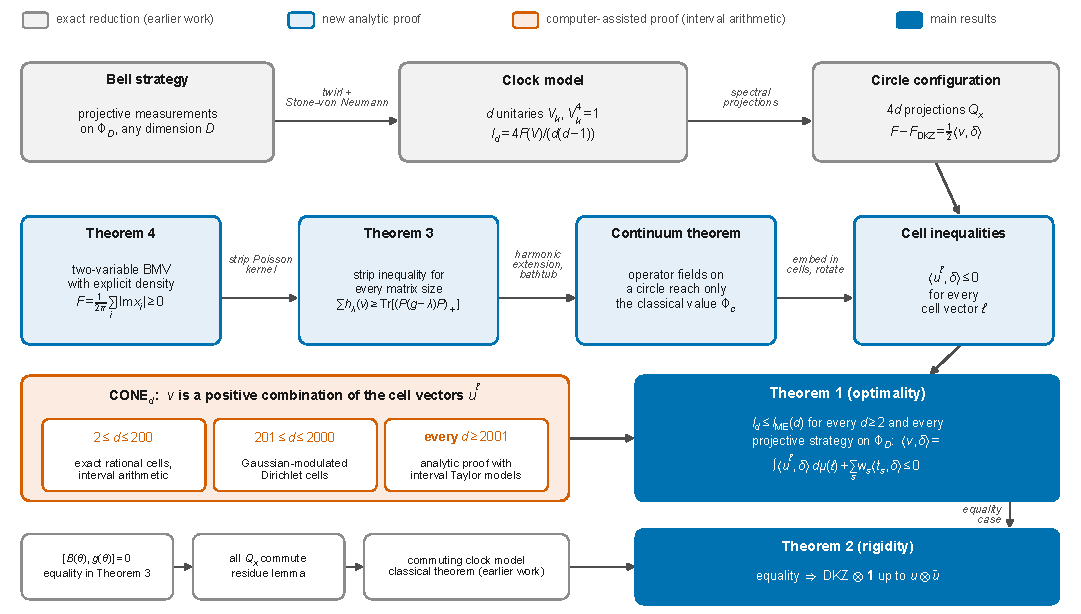
\includegraphics[width=\textwidth]{figures/fig2.pdf}
\caption{\textbf{Architecture of the proof.} Top row: exact reduction of a projective strategy on $\Phi_D$ to the clock
model~\eqref{eq:clock} and to a configuration of $4d$ projections on a circle, in which the deficit $F-\FD$ becomes the
linear form $\frac12\langle v,\delta\rangle$ of equation~\eqref{eq:linear} (Methods). Middle row: the new analytic
chain. Theorem~4 (an explicit positive density) implies Theorem~3 (the strip inequality, for matrices of every size);
Theorem~3 gives the continuum theorem for operator fields on a circle, and embedding the discrete configuration with
cells of lengths $\ell$ gives one linear inequality $\langle u^\ell,\delta\rangle\le0$ for every cell vector $\ell$.
Bottom: CONE$_d$, a statement about explicit Clausen-function kernels only, is certified for every $d$ in three regimes.
Together they give Theorem~1. Following the equality case through the chain gives Theorem~2.}
\label{fig:2}
\end{figure}

%==============================================================================================================
\section*{A matrix inequality on a strip}

The continuum theorem needs a single inequality between matrices. Let $B$ be an orthogonal projection on $\C^M$, let
$P=\one-B$, and let $g$ be Hermitian. The matrix $X=B+ig$ is not normal in general, but its eigenvalues lie in the strip
$0\le\Re\nu\le1$, because $\Re\langle\psi,X\psi\rangle=\langle\psi,B\psi\rangle$. On this strip let $h_\lambda$ be
the harmonic function with boundary values $(y-\lambda)_+=\max(y-\lambda,0)$ on the left edge and $0$ on the right
edge (Fig.~\ref{fig:3}b). It has the closed form
\begin{equation}\label{eq:h}
h_\lambda(x+iy)=-\frac{1}{\pi^2}\,\Im\Li\bigl(e^{\pi(y-\lambda)}e^{-i\pi x}\bigr),
\end{equation}
where $\Li$ is the dilogarithm.

\medskip
\noindent\textbf{Theorem 3 (strip inequality).} \emph{For every $M$, every orthogonal projection $B$ on $\C^M$, every
Hermitian $g$ and every real $\lambda$,
\begin{equation}\label{eq:strip}
\sum_{\nu\in\mathrm{spec}(B+ig)}h_\lambda(\nu)\;\ge\;\Tr\bigl[(P(g-\lambda)P)_+\bigr],
\end{equation}
where eigenvalues are counted with algebraic multiplicity and $(\cdot)_+$ is the positive part. Equality holds for one,
equivalently for all, $\lambda$ if and only if $B$ and $g$ commute.}
\medskip

\noindent If $B$ and $g$ commute, the eigenvalues of $B+ig$ lie on the edges of the strip: $i\mu$ for every eigenvalue
$\mu$ of $PgP$ on the range of $P$, and $1+i\mu'$ for every eigenvalue $\mu'$ of $BgB$ on the range of $B$. The boundary
values of $h_\lambda$ then turn the left side of~\eqref{eq:strip} into the right side exactly. If $B$ and $g$ do not
commute, the eigenvalues move into the interior (Fig.~\ref{fig:3}b), and the theorem says that this can only increase
the left side. There is an equivalent formulation that does not refer to $\lambda$. Sweep every eigenvalue $\nu$ to
the left edge with the harmonic measure of the strip, that is, replace it by the distribution of the point at which a
Brownian motion started at $\nu$ leaves the strip, counting only exits through the left edge (an eigenvalue with real
part $x$ contributes mass $1-x$). Theorem~3 states that the resulting distribution dominates the spectrum of the
compression $PgP$ in convex order\cite{Strassen1965} (Fig.~\ref{fig:3}a,c). It is thus a majorization theorem of
Schur--Horn type for non-normal matrices, with the Stein--Weiss theorem as its commutative case.

Before finding the general proof, we could establish Theorem~3 only in special cases, for instance for $M\le4$, by a
geometric argument based on Pedoe's inequality for polygons and independently by a Bellman-function argument. The
general case is the step from commuting to non-commuting measurements. Inequalities of this kind are delicate. Several
natural strengthenings, such as monotonicity of the left side along the path from the pinched matrix $BgB+PgP$ to $g$,
are false, with counterexamples already for $M=3$.

\begin{figure}[t]
\centering
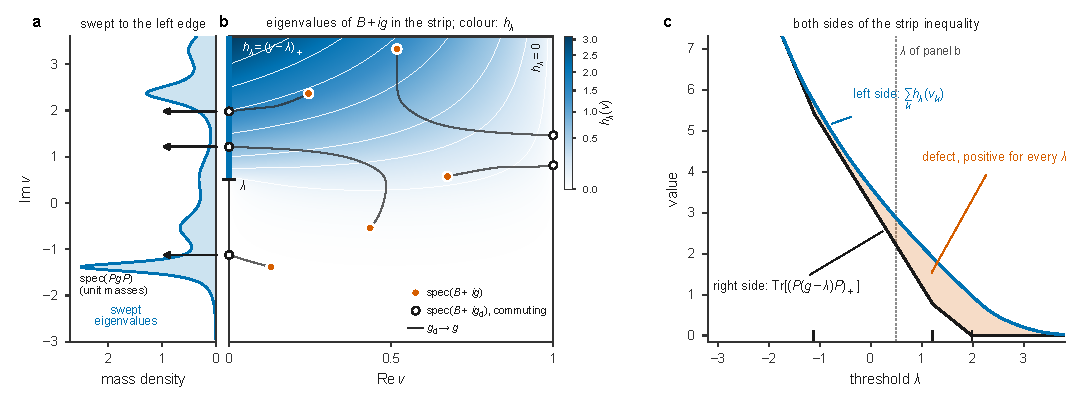
\includegraphics[width=\textwidth]{figures/fig3.pdf}
\caption{\textbf{The strip inequality.} A random example with $M=5$, $\mathrm{rank}\,B=2$ (seed fixed in the figure
script). \textbf{b}, The harmonic function $h_\lambda$ of equation~\eqref{eq:h} on the strip $0\le\Re\nu\le1$ for
$\lambda=0.5$ (colour; white contours), with boundary values $(y-\lambda)_+$ on the left edge (thick line) and $0$ on
the right edge. Orange dots: the eigenvalues of $B+ig$. Open circles: the eigenvalues for the pinched matrix
$g_{\rm d}=BgB+PgP$, which commutes with $B$; they lie on the edges, at the spectra of $PgP$ (left) and $BgB$ (right).
Thin lines: the eigenvalues of $B+i(g_{\rm d}+t(g-g_{\rm d}))$ for $0\le t\le1$. \textbf{a}, The eigenvalues of
$B+ig$ swept to the left edge by the harmonic measure of the strip (blue density, total mass $\mathrm{rank}\,P=3$),
compared with the three eigenvalues of $PgP$ (black spikes). Both have the same mass and the same mean. Theorem~3 says
that the blue distribution is more spread out, in the convex order. \textbf{c}, Both sides of
inequality~\eqref{eq:strip} as functions of $\lambda$. The right side (black) is piecewise linear with kinks at the
eigenvalues of $PgP$ (ticks). The defect (shaded) is positive for every $\lambda$; for the commuting pinched matrix
the two sides coincide.}
\label{fig:3}
\end{figure}

%==============================================================================================================
\section*{A hidden positive density}

Theorem~3 follows from an identity that exhibits its defect as an integral of a positive function. For complex $a$ and
$t$ consider the trace function
\begin{equation}\label{eq:D}
\mathcal{D}(a,t)=\Tr e^{ag-tP}-e^{-t}\,\Tr_P e^{aPgP}-\Tr_B e^{aBgB},
\end{equation}
in which the last two traces are over the ranges of $P$ and $B$. The first term is the trace of an exponential of two
non-commuting matrices; the other two are what it would be if $g$ were replaced by its pinching $BgB+PgP$. For fixed
$s\in\R$ and $0<\tau<1$ consider the matrix pencil $g-s-x(P-\tau)$ and its $M$ roots $x_1(s,\tau),\dots,x_M(s,\tau)$,
the values of $x$ at which it is singular.

\medskip
\noindent\textbf{Theorem 4 (two-variable BMV formula with an explicit density).} \emph{Let
\begin{equation}\label{eq:F}
F(s,\tau)=\frac{1}{2\pi}\sum_{i=1}^M\bigl|\Im x_i(s,\tau)\bigr|\qquad(s\in\R,\ 0<\tau<1).
\end{equation}
Then $F$ is continuous, non-negative and supported in $[\lambda_{\min}(g),\lambda_{\max}(g)]\times[0,1]$, and for all
complex $a,t$
\begin{equation}\label{eq:bmv2}
\mathcal{D}(a,t)=a^2\int_0^1\!\!\int_{\R}e^{as-t\tau}F(s,\tau)\,ds\,d\tau .
\end{equation}
Moreover, the defect of inequality~\eqref{eq:strip} is
\begin{equation}\label{eq:defect}
\sum_{\nu\in\mathrm{spec}(B+ig)}h_\lambda(\nu)-\Tr\bigl[(P(g-\lambda)P)_+\bigr]
=\int_0^1\!\!\int_\R K_{1-\tau}(s-\lambda)\,F(s,\tau)\,ds\,d\tau,
\end{equation}
where $K_X(u)=\sin(\pi X)/(2\cosh\pi u-2\cos\pi X)$ is the Poisson kernel of the strip.}
\medskip

\noindent For a projection $P$ and $a=1$, equation~\eqref{eq:bmv2} contains Stahl's theorem\cite{Stahl2013,Eremenko2015},
which settled the conjecture of Bessis, Moussa and Villani\cite{BMV1975,LiebSeiringer2004}: the function
$t\mapsto\Tr e^{A-tP}$ is the Laplace transform of a positive measure. Here the measure is explicit. It consists of
atoms $\Tr_Be^{BAB}$ at $\tau=0$ and $\Tr_Pe^{PAP}$ at $\tau=1$, plus the absolutely continuous part with density
$\int e^sF(s,\tau)\,ds$. The second variable $a$ and the subtraction of the pinched terms are what the strip inequality
needs, and positivity survives both. Theorem~4 is a statement about the positivity of a two-variable transform, so it
also yields the strip inequality~\eqref{eq:strip}, which involves functions that are not exponentials. Stahl's theorem
alone gives inequality~\eqref{eq:strip} only for exponential test functions.

Why should such a density exist, and why is it positive? The roots $x_i$ are the eigenvalues of
$(P-\tau)^{-1}(g-s)$, a matrix that is self-adjoint for an indefinite inner product, so they are real or come in
complex-conjugate pairs. For the pinched pencil all roots are real. The proof (Methods) reconstructs the distribution
$T$ whose Laplace transform is $\mathcal{D}/a^2$ from its one-dimensional projections, as in computed
tomography\cite{Natterer1986}. These projections are the differences between the eigenvalue distributions of $g-\xi P$
and of the pinched matrix, and filtered back-projection turns them into the logarithm of the ratio of the two
characteristic polynomials of the pencil. A Jensen-type identity shows that integrating this logarithm along a line
removes all real roots and leaves exactly $\pi\sum_i|\Im x_i|$. The density is therefore positive because
non-commutativity can only create complex pairs of roots, each of which contributes with a positive sign. A
Paley--Wiener argument\cite{Hormander1990} guarantees that $T$ exists and lives on a rectangle, and the behaviour of
$\mathcal{D}$ as $t\to\pm\infty$ excludes extra mass on the edges $\tau=0,1$, so $T=F$. A second, elementary proof
(Methods) obtains the projections of $F$ directly from a Burgers equation obeyed by the roots, without distributions;
it is the proof checked in Lean.

The same mechanism, a two-dimensional Fourier inversion of a trace of a pencil whose density is given by the imaginary
parts of pencil eigenvalues, was introduced by Hein\"avaara to give a new proof of Stahl's theorem\cite{Heinavaara2023}.
Theorem~4 is a variant adapted to a projection and to the pinched subtraction. We found it independently and learned of
the connection afterwards. Figure~\ref{fig:4} shows the density for the example of Fig.~\ref{fig:3}, the semicircle
laws that appear for $M=2$, and two independent numerical checks. The defect equals the strip transform of $F$ to
$1.4\times10^{-14}$, and every horizontal slice of $F$ has mass $\|BgP\|_F^2$, a sum rule that the proof does not use.

\begin{figure}[t]
\centering
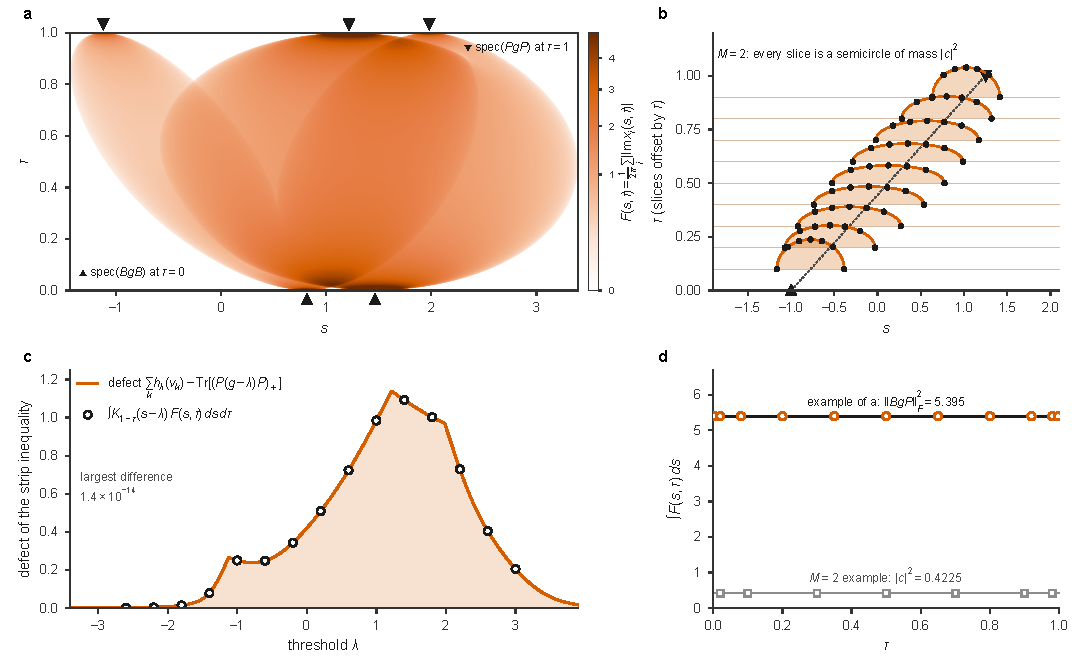
\includegraphics[width=\textwidth]{figures/fig4.pdf}
\caption{\textbf{The explicit positive density of Theorem~4.} \textbf{a}, $F(s,\tau)$ of equation~\eqref{eq:F} for
the example of Fig.~\ref{fig:3}, computed from the roots of the pencil $g-s-x(P-\tau)$ (colour scale compressed by a
square root). The density consists of lens-shaped sheets that connect the eigenvalues of $BgB$ at $\tau=0$ (triangles
below) with those of $PgP$ at $\tau=1$ (triangles above). \textbf{b}, For $M=2$, $B=\mathrm{diag}(1,0)$ and
$g=\bigl(\begin{smallmatrix}\alpha&c\\ \bar c&\beta\end{smallmatrix}\bigr)$, every slice is a semicircle law of radius
$2|c|\sqrt{\tau(1-\tau)}$ centred at $\tau\beta+(1-\tau)\alpha$ (shaded curves, offset by $\tau$; here $\alpha=-1$,
$\beta=1.25$, $c=0.65$); dots are the values computed from the roots. \textbf{c}, The defect of the strip
inequality for the example of panel a, computed from the eigenvalues of $B+ig$ and $PgP$ (line), and as the integral of
the density against the strip Poisson kernel (circles, adaptive quadrature); the largest difference is
$1.4\times10^{-14}$.
\textbf{d}, Every horizontal slice of the density has the same mass, $\int F(s,\tau)\,ds=\|BgP\|_F^2$ (circles: example
of panel a; squares: $M=2$, where the mass is $|c|^2$).}
\label{fig:4}
\end{figure}

%==============================================================================================================
\section*{From the strip back to the Bell inequality}

With Theorem~3 available for matrices of every size, the continuum problem can be solved. Let $B(\theta)$ be a
projection-valued function on the circle, let $0\le A(\theta)\le\one-B(\theta)$, and let $g$ be the conjugate function
(periodic Hilbert transform) of $B$. The \emph{continuum theorem} states that
\begin{equation}\label{eq:cont}
\int\tr\bigl(A(\theta)g(\theta)\bigr)\frac{d\theta}{2\pi}\;\le\;\Phi_c(\alpha,\beta)
=\frac{\Cl(2\pi\alpha)+\Cl(2\pi\beta)+\Cl(2\pi(1-\alpha-\beta))}{2\pi^2},
\end{equation}
where $\alpha$ and $\beta$ are the mean normalized traces of $A$ and $B$, and $\Cl$ is the Clausen function. The right
side is the value of two adjacent arcs, so in the continuum, matrix-valued configurations do no better than classical
ones. The proof (Methods) extends $B+ig$ to an analytic matrix function on the disc whose eigenvalues stay in the
strip, uses that the harmonic function $h_\lambda$ of these eigenvalues has the correct mean, applies Theorem~3 at every
point of the circle and finishes with the bathtub principle.

To return to the discrete problem, we embed the configuration of $4d$ projections into the continuous circle, giving the
site $x$ an arc whose length $\ell_x$ depends only on $x$ modulo $d$. The constraints of the Bell problem make every
such embedding admissible for the continuum theorem, and averaging over rotations turns
inequality~\eqref{eq:cont} into one linear inequality $\langle u^\ell,\delta\rangle\le0$ for the vector $\delta$ that
measures the deviation of the configuration from DKZ. The vector $u^\ell$ depends only on the cell lengths and is
given explicitly by Clausen functions (Methods). Equal cell lengths are not enough: the corresponding $u^\ell$ is not
proportional to the vector $v$ that defines $F-\FD$, and the difference is the junction effect that defeats a direct
continuum argument. Unequal cells repair this. Random cells, distributed like the gaps between uniform random
points on the circle, reproduce the singular part of the discrete kernel exactly, through a Bernstein-polynomial
identity (Methods), and leave a smooth residual of relative order $1/d$. What is needed, and what we prove, is
\begin{center}
CONE$_d$:\quad the vector $v$ is a positive combination of vectors $u^\ell$ with all cells of positive length
(and of trivially admissible directions).
\end{center}
Then $F-\FD=\frac12\langle v,\delta\rangle$ is a positive combination of quantities that the continuum theorem shows to
be non-positive, and Theorem~1 follows. CONE$_d$ involves only explicit special functions, with no operators and no
quantum mechanics.

We certify CONE$_d$ for every $d$ in three regimes (Fig.~\ref{fig:5}). For $2\le d\le200$ we give explicit rational
cell vectors (all cell lengths multiples of $1/16$) and positive weights, and verify the vector identity in interval
arithmetic with rigorous enclosures of the Clausen function. For $201\le d\le2000$ we use random cells whose Dirichlet
parameters are modulated by a stationary Gaussian process. The required identity then decouples into one scalar
equation per distance, its solution is enclosed in interval arithmetic for each $d$, and a Poincar\'e--Miranda
argument\cite{Kulpa1997} passes from the decoupled equations to the exact ones. Each of these $1800$ certificates is
produced by a single run of one checker at one precision, and every margin is certified on the Poincar\'e--Miranda box
itself. For $d\ge2001$ the same construction is treated analytically. The solution is approximated by a smooth model,
the fourth differences that control positivity are bounded by interval Taylor models on boxes that cover every
$d\ge2001$ at once, and the error of the model is bounded pointwise. All margins are large. The smallest certified
weights for $d\le200$ exceed $0.08/d$, the fixed-point derivative bound exceeds the required value by a factor of four
for every $201\le d\le2000$, and the normalized fourth differences for $d\ge2001$ are at least $6.02$ where $1/4$
suffices. A single audit script re-checks all three regimes.

\begin{figure}[tp]
\centering
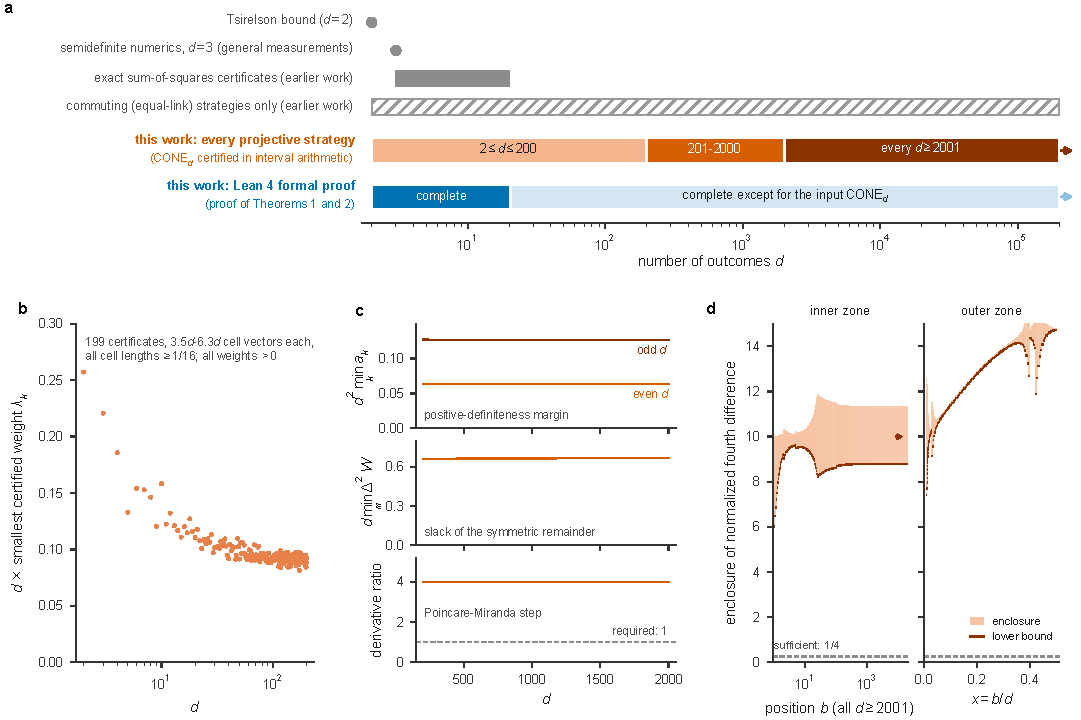
\includegraphics[width=\textwidth]{figures/fig5.pdf}
\caption{\textbf{Certification for every $d$.} \textbf{a}, Coverage of the optimality statement. Grey: earlier
results, namely Tsirelson's bound ($d=2$), semidefinite numerics for $d=3$ with general measurements\cite{LVN2014}, our
exact sum-of-squares certificates ($3\le d\le20$)\cite{repoCGLMP} and the commuting (equal-link) case for every
$d$\cite{classical2026} (hatched). Orange: the three regimes of the CONE$_d$ certificate, which together with
Theorem~3 give Theorem~1 for every $d$. Blue: the Lean formalisation of the proof of Theorems~1 and~2, complete for
$2\le d\le20$ and, for $d\ge21$, complete except for the input CONE$_d$ (Theorems~3 and~4 are formalised in full).
\textbf{b}, $2\le d\le200$: $d$ times the smallest certified weight of the exact cone certificate (rational cells,
interval arithmetic). \textbf{c}, $201\le d\le2000$: certified lower bounds, read from the single-run certificate of
each $d$ (160-bit interval arithmetic, every quantity enclosed on one Poincar\'e--Miranda box per $d$); plotted are the
lower endpoints of the certified enclosures of $d^2\min_ka_k$, the positive-definiteness margin of the Gaussian
modulation (top; even and odd $d$), of $d\min_m\Delta^2W$, the slack of the symmetric remainder (middle), and of the
derivative bound of the Poincar\'e--Miranda step divided by its required value (bottom; $1$ suffices). The smallest
values are $0.06319$ (even $d$), $0.12638$ (odd $d$), $0.660$ and $4.0009$. \textbf{d}, $d\ge2001$: interval enclosures
(bands) and certified lower bounds (lines) of the normalized fourth differences that control positivity, on the boxes
of the inner zone (positions $b\ge1$ with $b/d\le0.013$, for all $d\ge2001$ at once; the last box covers every
$b\ge1000$) and of the outer zone ($0.011\le b/d\le0.501$). Every lower bound lies far above the sufficient level
$1/4$.}
\label{fig:5}
\end{figure}

%==============================================================================================================
\section*{Rigidity}

Every step of the proof is an inequality with an explicit defect, so the equality case can be traced back through
the chain (Methods). If $I_d=\IME(d)$, the cone representation forces equality in a continuum inequality for an
embedding in which every cell has positive length. This forces equality in the strip inequality at almost every point
of the circle, so by the equality clause of Theorem~3 the matrices $B(\theta)$ and $g(\theta)$ commute almost
everywhere. Because $g$ is an explicit sum of logarithms of the distances to the cell endpoints, a residue argument then
shows that all $4d$ spectral projections commute. In the commuting case our classical theorem\cite{classical2026}
identifies the configuration as a direct sum of DKZ blocks, which gives Theorem~2. Theorem~2 extends to every $d$ the
rigidity that our exact certificates established for $3\le d\le20$\cite{repoCGLMP}; for those $d$ the two proofs are
independent.

%==============================================================================================================
\section*{The status of Open Quantum Problem 27}

Part~A of Open Quantum Problem~27 asked whether every facet of the local polytope is of CGLMP type; Bancal, Gisin and
Pironio answered it negatively\cite{BGP2010}. Part~B asks to show that the DKZ measurements are necessarily optimal on
maximally entangled states, that they give the highest resistance to noise, and that they are optimal for the
Kullback--Leibler discrimination of quantum from local correlations\cite{OQP27}. The clauses go back to Gill's numerical
observations\cite{Gill2007}. Table~\ref{tab:status} gives the verdict on each of them. Theorems~1 and~2 settle
optimality and uniqueness for every $d$.

The verdict on the noise clause depends on how noise resistance is measured. Mixing the correlations with uniformly
random outcomes of weight $1-v$ multiplies $I_d$ by $v$, so the smallest visibility at which the CGLMP inequality
detects nonlocality of a maximally entangled state is $2/\IME(d)$, and by Theorem~2 only the DKZ measurements reach it;
this consequence is also checked in Lean. Gill, however, asked for the violation of local realism, that is, of any Bell
inequality\cite{Gill2007}. In this literal reading the clause fails for every $d\ge4$ (Supplementary Information). A
strategy that uses the optimal two-outcome CHSH measurements, and never produces the other $d-2$ outcomes, tolerates
more noise than the DKZ measurements: the noise lands partly on the unused outcomes, and this helps the noisy
correlations to violate a coarse-grained CHSH inequality. We determine its critical visibility exactly, for
example $4(d-1)/((\sqrt2-1)d^2+4(d-1))$ for even $d$, and prove that the DKZ measurements need a higher one, with
computer-assisted certificates for $4\le d\le9$ and an elementary bound for $d\ge10$. The effect itself was noticed
before: Ac\'{\i}n, Durt, Gisin and Latorre found it for a two-qubit entangled state embedded in two qudits and concluded
that resistance to noise is not a good measure of nonlocality\cite{ADGL2002}, and Baek, Ryu and Lee observed it
numerically on maximally entangled states of local dimension 4 and 16\cite{BaekRyuLee2025}. As far as we found, the
general theorem and its bearing on Problem~27 are new. For $d=2$ the clause holds, and for $d=3$ it holds on $\Phi_3$
but fails on $\Phi_2$. The counterexample needs unused outcomes; whether DKZ is optimal when the noise acts on the state
and every outcome is used remains open; numerical searches support it for $d\le8$ (ref.~\citenum{GLZ2012} and
Supplementary Information).

The Kullback--Leibler clause\cite{vanDam2005} is false for every $d\ge4$: an explicit strategy built from pairs of CHSH
measurements has a statistical strength of at least $0.0703204$ bits, while that of the DKZ measurements is at most
$0.0687803$ bits in every dimension. Zhang found the first counterexample, for $d=4$\cite{Zhang2026}, and we gave
counterexamples for $4\le d\le9$ in earlier work\cite{repoCGLMP}. For $d=3$ the DKZ measurements are a strict local
maximum of the statistical strength; whether they are the global maximum is open. When the state may also be chosen,
the best tests use states that are not maximally entangled\cite{AGG2005}.

\begin{table}[t]
\centering\small
\caption{\textbf{Status of Open Quantum Problem 27.} ``Max-ent'' refers to maximally entangled states of any local
dimension. The positive statements concern projective measurements; the counterexamples use projective measurements.}
\label{tab:status}
\begin{tabular}{>{\raggedright\arraybackslash}p{5.3cm}>{\raggedright\arraybackslash}p{9.6cm}}
\toprule
clause & status\\
\midrule
27A: all facets of the local polytope of CGLMP type & false\cite{BGP2010}\\
27B: DKZ optimal on max-ent states & proved for every $d$ (Theorem~1), with a computer-assisted step for $d\ge21$; fully
formalised in Lean for $d\le20$; earlier: $3\le d\le20$ and the commuting case for every
$d$\cite{repoCGLMP,classical2026}\\
27B: DKZ unique (rigidity) & proved for every $d$ (Theorem~2), with the same computer-assisted step for $d\ge21$; fully
formalised in Lean for $d\le20$; earlier: $3\le d\le20$\cite{repoCGLMP}\\
27B: highest noise resistance, CGLMP inequality, uniformly random outcomes as noise & true for every $d$, DKZ the
unique optimum (Theorems~1 and~2; formalised in Lean with the same scope)\\
27B: highest noise resistance, all Bell inequalities, uniformly random outcomes as noise (Gill's reading) & false for
every $d\ge4$ (Supplementary Information); true for $d=2$; $d=3$: true on $\Phi_3$, false on $\Phi_2$\\
strengthening: white noise on the state, every outcome used & open for $d\ge4$; DKZ optimal in numerical searches for
$d\le8$\\
27B: optimal Kullback--Leibler discrimination & false for every $d\ge4$ (Supplementary Information; $d=4$ first in
ref.~\citenum{Zhang2026}); $d=3$: DKZ a strict local maximum\\
maximal value over all states & exact for $3\le d\le8$\cite{IoannouRosset2021,repoCGLMP}; open for $d\ge9$\\
\bottomrule
\end{tabular}
\end{table}

%==============================================================================================================
\section*{Discussion}

We have shown that the DKZ measurements are the optimal and essentially unique projective measurements for the CGLMP
inequality on maximally entangled states, in every dimension. This settles the clause of IQOQI Open Quantum Problem~27B
that asks for necessity on maximally entangled states, which had been supported by numerics for more than two decades.
Together with the negative answer to Part~A\cite{BGP2010} and our verdicts on the noise and Kullback--Leibler clauses
(Table~\ref{tab:status}), this completes the resolution of Open Quantum Problem~27 as originally posed, with the verdict
on the noise clause depending on its reading. The proof uses a computer only for the certificate CONE$_d$, in interval arithmetic, and for $d\le20$ it is checked in
full by the Lean theorem prover. An analytic proof of CONE$_d$ would remove the computer-assisted step and, once
formalised, complete the formal proof for every $d$.
For experiments, Theorem~1 provides the exact benchmark $\IME(d)$ for maximally entangled sources of every dimension.
Theorem~2 shows that projective measurements that reach the benchmark on a maximally entangled source are equivalent to
DKZ, the starting point for certifying high-dimensional measurements from the observed statistics. A quantitative
version of Theorem~2 would bound the distance to DKZ in terms of the gap $\IME(d)-I_d$. Our proof suggests a route: it
expresses the gap exactly as a positive combination of integrated defects of the strip inequality and of explicit
non-negative slack terms, and Theorem~4 expresses each defect as an integral of a positive density that vanishes only
in the commuting case. Such a bound is what applications to randomness
certification and robust self-testing would require\cite{SupicBowles2020,Pironio2010}.

Three questions remain. The first concerns general measurements. Our statements cover projective measurements, which
is the setting of the original question. A general measurement on $\Phi_D$ can be realized as a projective measurement
on a larger space, but the enlarged state is then no longer maximally entangled, so the extension is not automatic. The
second concerns the optimal state. The maximal CGLMP value over all states is attained by states that are not maximally
entangled\cite{ADGL2002}, and it is known exactly only for $d\le8$. Our reduction extends to every pure state as a
clock model with site-dependent weights (we do not give the details here). Whether the cone method extends to it is
open. The third is the noise clause with white noise on the state and every outcome used, which is open for $d\ge4$.

The mathematical tools may be useful beyond Bell inequalities. The strip inequality is a majorization principle for
non-normal matrices whose real part is a projection. It connects the eigenvalues of $B+ig$ with the spectrum of a
compression, and it reduces to the Stein--Weiss theorem in the commutative case. Theorem~4 shows that a two-variable,
pinched version of the Bessis--Moussa--Villani formula has a positive density that can be written down explicitly,
which complements the abstract positivity of Stahl's theorem\cite{Stahl2013,Heinavaara2023}. The continuum value
$\Phi_c$ in equation~\eqref{eq:cont} is the volume of an ideal hyperbolic tetrahedron with dihedral angles
$\pi\alpha,\pi\beta,\pi(1-\alpha-\beta)$ divided by $\pi^2$\cite{Milnor1982}, and up to the factor $-1/\pi$ it coincides
with the surface tension of lozenge tilings\cite{KOS2006}. We do not know whether these coincidences have a deeper meaning for Bell
inequalities.

%==============================================================================================================
\section*{Methods}

\subsection*{CGLMP expression and maximally entangled strategies}
We use equation~\eqref{eq:cglmp}, in which $P(A_x=B_y+k)$ means $A_x-B_y\equiv k\pmod d$. This is the reading under
which local models obey $I_d\le2$ and the DKZ measurements give $\IME(d)$\cite{CGLMP2002}. For projective measurements
on $\Phi_D$ one has $P(a,b|x,y)=\tau(P^x_a(Q^y_b)^{\mathsf T})$ with $\tau=\frac1D\Tr$ and the transpose taken in the
Schmidt basis of $\Phi_D$. With $w=e^{2\pi i/d}$, $U_x=\sum_aw^aP^x_a$ and $U'_y=\sum_bw^bQ^y_b$, put $R_1=U_2$,
$R_2=(U'_2)^{\mathsf T}$, $R_3=U_1$ and $R_4=(U'_1)^{\mathsf T}$. These are unitaries with $R_i^d=\one$. The
Fourier expansion of the residue function $m(t)\in\{0,\dots,d-1\}$ gives
\begin{equation}\label{eq:Strace}
I_d=4-\frac{2S}{d-1},\qquad S=2(d-1)+\sum_{n=1}^{d-1}c_n\sum_{i=0}^{3}\tau\bigl(L^{(i)}_n\bigr),\qquad
c_n=-\frac{1}{1-w^{-n}},
\end{equation}
with the links $L^{(0)}_n=R_1^nR_2^{-n}$, $L^{(1)}_n=R_2^nR_3^{-n}$, $L^{(2)}_n=R_3^nR_4^{-n}$ and
$L^{(3)}_n=w^{-n}R_4^nR_1^{-n}$. Conversely, any four unitaries with $R_i^d=\one$ define a projective strategy on
$\Phi_D$ through their spectral projections\cite{classical2026}.

\subsection*{Reduction to the clock model}
Let $z=e^{2\pi i/4d}$. The map $\rho(R_1,R_2,R_3,R_4)=(R_2,R_3,R_4,wR_1)$ leaves $S$ invariant, and since $\rho^4$
multiplies every $R_i$ by $w$ (which also leaves $S$ invariant), it generates a cyclic group of order $4d$. The direct
sum $\tilde R=\bigoplus_{r\in\Z_{4d}}\rho^r(R)$ has
the same value and contains $R$ as a direct summand. The cyclic shift of the summands is a unitary $W$ with
$W\tilde R_iW^\dagger=\tilde R_{i+1}$ ($i=1,2,3$), $W\tilde R_4W^\dagger=w\tilde R_1$ and $W^{4d}=\one$. Then
$Z=W^4$ satisfies $Z\tilde R_1Z^\dagger=w\tilde R_1$ and $Z^d=\one$. By the Stone--von Neumann theorem for $\Z_d$,
$\tilde R_1=X\otimes\one_M$ and $Z=Z_0\otimes\one_M$, with $X$ the cyclic shift and $Z_0$ the clock matrix on $\C^d$.
Since $W$ commutes with $Z$, $W=\sum_k|k\rangle\langle k|\otimes z^kV_k$ with $V_k^4=\one$. Inserting this
\emph{covariant} form into equation~\eqref{eq:Strace} gives equation~\eqref{eq:clock}; conversely every family $V$
defines the covariant strategy $R^V_1=X\otimes\one$, $R^V_{i+1}=WR^V_iW^\dagger$ on $\C^d\otimes\C^M$. The DKZ
strategy is, up to the local unitary $W_0^{-2}\otimes\overline{W_0^{-2}}$ with $W_0=\mathrm{diag}(z^k)$, the covariant
strategy with $M=1$ and $V\equiv1$. Full proofs are in ref.~\citenum{classical2026} (Theorem~2.3 and its appendix).

\subsection*{The circle configuration and the linear form}
Let $N=4d$ and $E_k=V_k^\dagger$. Every $x\in\Z_N$ can be written uniquely as $x=k-da$ with $0\le k\le d-1$ and
$a\in\Z_4$; let $Q_x$ be the spectral projection of $E_k$ for the eigenvalue $i^a$. For every site $k$ the four
projections $Q_{k-da}$ form a projective measurement. Put $A_x=Q_x$, $B_x=Q_{x+d}$, $\kappa(u)=\cot(\pi u/N)$
($\kappa(0)=0$), $T(m)=\sum_y\tau(A_{y+m}B_y)$ and $N(m)=T(m)-T(-m)$. Then $F(V)=\frac12\sum_{x,y}\kappa(x-y)\tau(A_xB_y)
-\frac d2$. Using $N(d)=d$ and $N(2d-m)=N(m)$, one finds
\begin{equation}\label{eq:linear}
F(V)-\FD=\tfrac12\langle v,\delta\rangle,\qquad v_m=2\csc\frac{\pi m}{2d},\qquad\delta_m=N(m)-m\qquad(1\le m\le d-1).
\end{equation}
The DKZ configuration is a pair of adjacent blocks and has $\delta=0$. For $1\le s\le d-1$ an elementary count gives
$\delta_s+\delta_{d-s}\le0$, so the directions $t_s=e_s+e_{d-s}$ are trivially admissible.

\subsection*{Proof of Theorems 3 and 4}
We write $g_{\rm d}=BgB+PgP$ and $p_{s,\tau}(x)=\det(g-s-x(P-\tau))$, $q_{s,\tau}(x)=\det(g_{\rm d}-s-x(P-\tau))$.
Complete proofs are in the Supplementary Information; here we list the steps.
(i)~\emph{Pencil facts.} For $0<\tau<1$ every root of $p_{s,\tau}$ satisfies $|x|\le\|g-s\|/\min(\tau,1-\tau)$, and
every non-real root satisfies $|x|\le\|g-s\|/\sqrt{\tau(1-\tau)}$ (a non-real root has an eigenvector $\psi$ with
$\langle\psi,(P-\tau)\psi\rangle=0$). All roots are real if $s\notin(\lambda_{\min},\lambda_{\max})$, all roots of
$q_{s,\tau}$ are real, and $p_{s,\tau}$, $q_{s,\tau}$ have the same leading coefficient and the same sum of roots.
Hence $F$ is continuous, bounded by $(M/2\pi)\|g-s\|/\sqrt{\tau(1-\tau)}$, and compactly supported.
(ii)~\emph{Jensen-type identity.} If $p$ and $q$ have degree $M$, the same leading coefficient and the same sum of
roots, and $q$ has only real roots, then $\int_\R\log|p(\xi)/q(\xi)|\,d\xi=\pi\sum_i|\Im x_i|$, the sum over the roots
of $p$. This follows from $\int_\R\frac12\log(1+b^2/u^2)\,du=\pi|b|$.
(iii)~\emph{A distribution with Laplace transform $\mathcal{D}/a^2$.} $\mathcal{D}(0,t)=\partial_a\mathcal{D}(0,t)=0$,
so $G=\mathcal{D}/a^2$ is entire on $\C^2$, and $|\mathcal{D}(a,t)|\le2M\exp\max_{(s,\tau)\in K}(s\Re a-\tau\Re t)$ with
$K=[\lambda_{\min},\lambda_{\max}]\times[0,1]$. By the Paley--Wiener--Schwartz theorem\cite{Hormander1990} there is
a distribution $T$ supported in $K$ with $T(e^{as-t\tau})=G(a,t)$.
(iv)~\emph{Fourier slices.} On the line $t=a\xi$, $G(a,a\xi)$ is the Laplace transform of the piecewise linear function
$U_\xi(w)=\sum_j[(w-\lambda_j(\xi))_+-(w-\lambda^0_j(\xi))_+]$, where $\lambda_j(\xi)$ and $\lambda^0_j(\xi)$ are the
eigenvalues of $g-\xi P$ and $g_{\rm d}-\xi P$. The Hilbert transform of $U_\xi'$ is
$\frac1\pi\log|\det(g-\xi P-w)/\det(g_{\rm d}-\xi P-w)|$, which at $w=s-\xi\tau$ equals
$\frac1\pi\log|p_{s,\tau}(\xi)/q_{s,\tau}(\xi)|$. Fourier inversion in polar coordinates (the Fourier slice
theorem\cite{Natterer1986}) integrates this over all lines through $(s,\tau)$, and step~(ii) gives $T=F$ on the open
strip $0<\tau<1$.
(v)~\emph{No mass on the edges.} $T-F$ is supported on $\tau\in\{0,1\}$. By the structure theorem for distributions
supported on a line, its Laplace transform is $\sum_kt^k[A_k(a)+e^{-t}B_k(a)]$. The limits
$\lim_{t\to+\infty}\Tr e^{ag-tP}=\Tr_Be^{aBgB}$ and $\lim_{t\to-\infty}e^t\Tr e^{ag-tP}=\Tr_Pe^{aPgP}$ force all $A_k$
and $B_k$ to vanish. Hence $T=F$, which is equation~\eqref{eq:bmv2}.
(vi)~\emph{Strip inequality.} $h_\lambda(x+iy)=\int(w-\lambda)_+K_x(y-w)\,dw$ is the Poisson integral of its boundary
values, and $\int e^{-au}K_X(u)\,du=\sin(a(1-X))/\sin a$ for $|\Re a|<\pi$. Let $\rho$ be the sum over the eigenvalues
$\nu_k=x_k+iy_k$ of $B+ig$ of the harmonic measures $K_{x_k}(y_k-w)\,dw$, and $\sigma$ the eigenvalue counting measure
of $PgP$. For $0<|a|<\pi$, the Laplace transform of $\rho$ is $[\Tr e^{ag+iaP}-\Tr e^{ag-iaP}]/(2i\sin a)$, and that
of $\sigma$ is $\Tr_Pe^{aPgP}$. By equation~\eqref{eq:bmv2} at $t=\mp ia$ the difference is the Laplace transform of
$a^2V$, where $V(w)=\int_0^1\!\int K_{1-\tau}(s-w)F(s,\tau)\,ds\,d\tau\ge0$. Matching moments then shows that the
defect of~\eqref{eq:strip} equals $V(\lambda)$. If the defect vanishes for one $\lambda$, then $F\equiv0$, hence
$\mathcal{D}\equiv0$, and the second-order term $\mathcal{D}(a,t)=a^2\|BgP\|_F^2(1-e^{-t})/t+O(a^3)$ gives $BgP=0$,
that is, $[B,g]=0$.
(vii)~\emph{An elementary route.} Steps (iii)--(v) can be replaced by an argument without distributions, Paley--Wiener
theory or Fourier inversion. It rests on a Radon identity: for Hermitian $H$, with $y_i(\tau)$ the eigenvalues of
$(P-\tau)^{-1}H$,
\begin{equation}\label{eq:RI}
\frac1{2\pi}\int_0^1\sum_i\bigl|\Im y_i(\tau)\bigr|\,d\tau=\Tr H_+-\Tr\bigl(BHB+PHP\bigr)_+ .
\end{equation}
To prove it, shift $H$ to $H+c$ with $\Im c>0$. Then no root is real and exactly $\mathrm{rank}\,P$ roots lie in the
upper half-plane, and the roots obey the complex inviscid Burgers equation $\partial_\tau y=y\,\partial_cy$, so that
$\partial_\tau\sum\mathrm{Log}\,y=\partial_c\sum y$ for the roots in the upper half-plane (a Cauchy integral, valid also
at repeated roots). Integrating over $\tau$, evaluating the two ends by a Schur complement, and letting $c$ tend to the
real axis gives equation~\eqref{eq:RI}. Applied to $H=g-\xi P-w$, it says that the integral of $F$ along the line
$s=w+\xi\tau$ equals $U_\xi(w)$. Tonelli's theorem for real $a$ and $t$ and the identity theorem for entire functions
then give equation~\eqref{eq:bmv2} on $\C^2$, and in step~(vi) the uniqueness of the Laplace transform is needed only for
continuous, exponentially decaying functions of one variable. This is the route followed by the Lean formalisation,
which uses the Fourier inversion theorem of Mathlib for that one-variable step. The same argument for an arbitrary
Hermitian matrix in place of $P$ gives a proof of Stahl's theorem\cite{Stahl2013} without distribution theory or Fourier
analysis; we make no priority claim about this by-product.

\subsection*{The continuum theorem}
Let $B(\theta)$ be a projection-valued step function on the circle (step functions are all that the cell embeddings
need), $0\le A(\theta)\le\one-B(\theta)$, and $g$ the entrywise conjugate function of $B$. The Herglotz integral $H(z)=\int\frac{e^{i\phi}+z}{e^{i\phi}-z}B(\phi)\frac{d\phi}{2\pi}$
is analytic on the unit disc with boundary values $B+ig$, and its numerical range, hence its spectrum, lies in the strip.
The function $\phi_\lambda(w)=\frac{i}{\pi^2}\Li(e^{-i\pi w-\pi\lambda})$ is analytic on the strip with
$\Re\phi_\lambda=h_\lambda$, so $z\mapsto\Re\Tr\phi_\lambda(H(z))=\sum_{\nu\in\mathrm{spec}\,H(z)}h_\lambda(\nu)$ is
harmonic. By the mean-value property and dominated convergence, its boundary mean equals its value at the centre,
$\sum_ih_\lambda(\beta_i)$ over the eigenvalues $\beta_i$ of $\int B$, which is at most $Mh_\lambda(\beta)$ because
$x\mapsto h_\lambda(x)$ is concave on $[0,1]$. With Theorem~3 at
every boundary point and $\tau(A(g-\lambda))\le\tau((P(g-\lambda)P)_+)$ this gives
$\int\tau(Ag)\le\lambda\alpha+h_\lambda(\beta)$ for every $\lambda$. Minimizing over $\lambda$ gives $\Phi_c(\alpha,\beta)$
by a Legendre identity for the dilogarithm. For $\alpha=\beta=\frac14$ the minimizer is $\lambda^*=\log2/(2\pi)$ and
$\Phi_c(\frac14,\frac14)=G/\pi^2$.

\subsection*{Cell embeddings and CONE$_d$}
A cell vector is $\ell\in\R^d$ with $\ell_r\ge0$ and $\sum_r\ell_r=d$, extended $d$-periodically to $\Z_N$. Give the
site $x$ the arc $I_x=[L_x,L_{x+1})$ of length $\ell_x$ on the circle $\R/N\Z$, and let $\tilde A,\tilde B$ be the step
functions equal to $A_x,B_x$ on $I_x$. Because $\ell$ depends only on the residue modulo $d$ and every residue class
carries a projective measurement, $\int\tilde B=\int\tilde A=d\,\one$. The continuum theorem therefore gives
$\sum_{x,y}K^\ell(x,y)\tau(A_xB_y)\le N^2\Phi_c(\frac14,\frac14)$, with
$K^\ell(x,y)=\int_{I_x}\int_{I_y}\cot(\pi(\xi-\eta)/N)\,d\xi\,d\eta$, and equality for every DKZ block. Averaging over
the $d$ rotations of the configuration gives $\langle u^\ell,\delta\rangle\le0$ with
\begin{equation}\label{eq:ul}
u^\ell_m=\Delta^2_m\,\frac1d\sum_{r=0}^{d-1}\hat G\bigl(\ell_r+\dots+\ell_{r+m-1}\bigr),\qquad
\hat G(u)=G(u)+G(2d-u),\quad G(u)=-\frac{N^2}{2\pi^2}\Cl\Bigl(\frac{2\pi u}{N}\Bigr),
\end{equation}
where $\Delta^2_m$ is the second difference in $m$, while $v_m=\hat G''(m)$. CONE$_d$ is the statement that
$v=\int u^\ell\,\mu(d\ell)+\sum_sw_st_s$ for a finite positive measure $\mu$ carried by cell vectors with all cells
positive and numbers $w_s\ge0$; in particular $v$ lies in the convex cone generated by the vectors $u^\ell$ and the
trivial directions $t_s$. For cells distributed as $d$
times a Dirichlet$(1,\dots,1)$ vector, the window sums are Beta-distributed, and the Bernstein derivative formula gives
$\Delta^2_m\mathbb{E}\,\phi(S(m))=\frac{d}{d+1}\mathbb{E}\,\phi''(dX)$ with $X\sim\mathrm{Beta}(m+1,d-m+1)$. This
reproduces the $1/u$ singularity of $\hat G''$ exactly and leaves a smooth residual of relative order $1/d$, which is
what the three regimes below correct.

\subsection*{Certification of CONE$_d$}
\emph{$2\le d\le200$.} For every $d$ we give $K\approx3.5d$--$6.3d$ cell vectors $\ell^{(k)}=n^{(k)}/16$ with integers
$n^{(k)}_r\ge1$ and $\sum_rn^{(k)}_r=16d$, and weights $\lambda_k$ with $\sum_k\lambda_ku^{\ell^{(k)}}=v$. All window
sums are multiples of $1/16$, so $\hat G$ is needed only on a grid. Each Clausen value is enclosed in 160-bit interval
arithmetic\cite{mpmath,Tucker2011} by its Bernoulli series with an explicit tail bound. The weights come from a
floating-point linear program\cite{HiGHS2018}; the exact solution of the linear system is enclosed by a residual bound,
and every weight is certified positive (smallest $4.25\times10^{-4}$, at $d=198$; $d$ times the smallest weight is at
least $0.0816$). A complete re-verification of all 199 certificates passed. Independent floating-point re-evaluations
of the identity at selected $d$, with 50-digit Clausen values and, for small $d$, the original cell-pair kernel, agree
to the precision of the stored weights. For $d\le20$ the same certificates are re-evaluated by the Lean kernel in exact
rational interval arithmetic.

\emph{$201\le d\le2000$.} Let $\eta$ be a centred stationary Gaussian vector on $\Z_d$ whose covariance is the second
difference of a variogram $\Phi$, and let $\ell=d\cdot\mathrm{Dirichlet}(1+\eta)$ on the event $\max_r|\eta_r|<\frac34$
(uniform Dirichlet otherwise). The cone identity reduces to two conditions: an antisymmetric part, which decouples up to
an error $e^{-cd}$ into one scalar equation per distance $m<d/2$, and a symmetric remainder whose second differences
must be non-negative. A Poincar\'e--Miranda argument on a box around the solution $\Phi_*$ of the decoupled equations
then produces an exact solution. For each $d$, a single run of one checker certifies all of this: in 160-bit interval
arithmetic throughout, with one code version (its SHA-256 hash is stored in every certificate), it encloses $\Phi_*$
(an exact order-14 Gaussian expansion with an order-16 remainder), fixes one Poincar\'e--Miranda box, and certifies on
that widened box that every Fourier coefficient $a_k$ of the variogram is positive (so that it defines a covariance),
that the symmetric remainder is positive, that the derivative bound and the sign conditions on the faces of the box
hold, and that the Gaussian tail $\epsilon_{\rm t}$ is negligible. Factorials, binomial coefficients and Bernoulli
numbers are exact, the zeta values are enclosed by the Euler--Maclaurin formula with a rigorous remainder, and no
decision is taken on floating-point numbers. An audit script re-checks all 1800 certificates from the stored exact
values (1800 of 1800 pass). The smallest certified margins are $d^2\min_ka_k\ge0.06319$ (even $d$) and $\ge0.12638$
(odd $d$), $d\min_m\Delta^2W\ge0.660$ for the symmetric remainder, a derivative bound $4.0009$ times the required value,
face margins above $10^{16.7}$ times the required $2\epsilon_{\rm t}$, and $\epsilon_{\rm t}\le10^{-31.16}$.

\emph{$d\ge2001$.} The same process is analyzed for all $d\ge2001$ at once, with $\epsilon=1/d$. A smooth model $\Phi_e$
is defined through the root of a quartic equation with explicit special-function coefficients. Its fourth
differences, which control the positive definiteness through a Fej\'er--P\'olya argument, are enclosed by interval
Taylor models in $(x,\epsilon)$ on boxes covering $0.011\le x\le0.501$ (outer zone, lower bound $7.419$) and all stencil
positions with $x\le0.013$ (inner zone, lower bound $6.022$). Separate bounds hold at the first two stencil positions.
The decoupled solution differs from the model by at most $6.6468\times10^{-4}\epsilon^2$ pointwise, which yields
$a_k\ge0.1186944\,w_k\epsilon^2$ for all $k$ and $\Delta^2W\ge0.620154\,\epsilon$ for the symmetric remainder; the tail
and fixed-point conditions hold with logarithmic margins above $800$. The constants entering these bounds, such as the
Fej\'er--P\'olya constant $0.1054878997577$, are themselves computed in interval arithmetic. A final rigour pass completed
the written proofs of the model identities and corrected some code-level enclosure defects, one of which had left a
sliver of size about $10^{-20}$ of the parameter range uncovered at $d=2001$; no conclusion changed. One command re-checks
all three regimes (the coverage of every box and every margin) and reports CONE$_d$ certified for every $d\ge2$.

\subsection*{Rigidity}
Let $I_d=\IME(d)$, so $\langle v,\delta\rangle=0$. In the cone representation every term is non-positive, so
$\langle u^\ell,\delta\rangle=0$ for a cell vector $\ell$ with all cells positive. Every certificate contains such
vectors: for $d\le200$ all cells are at least $1/16$, and for $d>200$ the Dirichlet law charges only the open simplex.
Then every rotated continuum inequality is tight. Following the continuum proof, equality forces equality in
Theorem~3 at $\lambda^*$ for almost every $\theta$, hence $[B(\theta),g(\theta)]=0$ almost everywhere. On each open arc
$I_x$, $g(\theta)=\frac1\pi\sum_j(B_j-B_{j-1})\log|\sin\frac{\theta-t_j}{2}|$ is real-analytic, with distinct endpoints
$t_j$. Differentiating $[B_x,g(\theta)]=0$ and comparing the residues at the poles $t_j$ shows that $[B_x,B_j]$ does not
depend on $j$; it therefore vanishes, so all $Q_x$ commute. Then the $V_k$ commute, the strategy has equal links, and
Theorem~B and Corollary~C of ref.~\citenum{classical2026} identify it as $\mathrm{DKZ}\otimes\one$ up to $u\otimes\bar u$.

\subsection*{Independent verification}
Four independent verifications were carried out. In each, an independent checker re-derived the proof step by step,
including all signs and conventions, and wrote the numerical checks from scratch; the reports are in the repository.
(1)~Theorems~3 and~4 by the Fourier-slice route: correct. The independent re-implementation confirms
equation~\eqref{eq:bmv2} at 82 complex points $(a,t)$ to $6.8\times10^{-13}$ and the defect formula at 51 pairs of
instance and $\lambda$ to $1.3\times10^{-12}$, including adversarial configurations with spectra up to $\pm150$ and
clustered eigenvalues. (2)~The elementary proof of the Radon identity (step~(vii) above): correct; the identities were
confirmed to 34--46 digits. (3)~The reduction chain, the continuum theorem, the cell inequalities, the logic of
CONE$_d$ and the rigidity argument: correct. (4)~A second proof of Theorem~3 for $\mathrm{rank}\,B\le1$, which also
covers $\mathrm{corank}\,B\le3$ and hence all $M\le5$, by a one-dimensional reduction and the argument principle:
correct (no mathematical error; some expository gaps, none of which changes a statement). In addition, for $d\le200$ the CONE$_d$ certificates are checked by a script separate from the one that
produced them, in all three regimes the rigorous computations agree with independent floating-point computations, and
the rigidity chain was tested numerically on step fields and random non-commuting configurations. For $3\le d\le20$,
Theorems~1 and~2 were proved earlier by exact sum-of-squares certificates that use neither Theorem~3 nor
CONE$_d$\cite{repoCGLMP}. The results on the remaining clauses were checked in the same way: the theorem on the
literal noise clause by two independent checkers, and the Kullback--Leibler theorem by one; no error was found.

\subsection*{Formal verification}
The argument is formalised in the Lean~4 theorem prover (version 4.33.1) with its mathematical library Mathlib
(revision 0df444a)\cite{Lean2021,Mathlib2020}, in 96 files of about 33,000 lines. No file uses \texttt{sorry},
\texttt{admit}, an \texttt{axiom} declaration or \texttt{native\_decide}, and every main theorem depends only on the
three standard axioms of Lean (\texttt{propext}, \texttt{Classical.choice}, \texttt{Quot.sound}). The main formal
theorems state the following. For every $2\le d\le20$, Theorems~1 and~2 and the value of the DKZ strategy hold, with no
assumption (\nolinkurl{OQP27.maxEntClause_le_twenty}). For every $d\ge2$, Theorems~1 and~2 hold, assuming only
CONE$_d$ for $d\ge21$ (\nolinkurl{OQP27.maxEntClause_all}). Theorem~3 with its equality
case, Theorem~4 with the defect formula, and the Radon identity~\eqref{eq:RI} hold for every matrix size, with no
assumption; the continuity of $F$, the sum rule of Fig.~\ref{fig:4}d and the dilogarithm formula~\eqref{eq:h}, which the
formal proof does not need, are proved on paper only. The formal rigidity statement asserts that $d$ divides $D$ and that
a unitary $u$ maps the measurements to $\mathrm{DKZ}\otimes\one$; the uniqueness of $u$ and the case $d\nmid D$ follow by
short arguments on paper. The remaining
formal theorems, all without assumptions, are the exact reduction from strategies to the linear
form~\eqref{eq:linear}, the continuum theorem for step fields (with explicit Herglotz functions), which gives every cell
inequality, the classical (commuting) theorem for every $d$, the DKZ value for every $d$, and CONE$_d$ for
$2\le d\le20$, whose explicit certificates are re-evaluated by the Lean kernel in exact rational interval arithmetic by
a checker that is itself proved sound. Hence the maximally entangled clause of Open Quantum Problem~27B is fully
machine-checked for $2\le d\le20$, and for $d\ge21$ the formal proof is complete except for the single input CONE$_d$,
which is established by the interval-arithmetic certificates described above, outside Lean. In Lean, CONE$_d$ is stated
as a finite positive combination of cell vectors that includes a cell vector with all cells positive; for $d\ge201$ this
finite form follows from the integral form produced by the certificates by Carath\'eodory's theorem, the trivial
directions being realized by cells supported on two residues. The consequence for the CGLMP noise threshold
(Table~\ref{tab:status}) is formalised in a further file, \texttt{CglmpNoise.lean}, with the same assumptions as
Theorems~1 and~2 and the same three axioms.

\subsection*{The noise and Kullback--Leibler clauses}
Let $u(a,b|x,y)=d^{-2}$ be the behaviour of uniformly random outcomes, and let $v_{\rm c}(p)$ be the largest $v$ for
which $vp+(1-v)u$ is local. For even $d$ the competitor measures the optimal CHSH observables on the factor $\C^2$ of
$\Phi_d=\Phi_2\otimes\Phi_{d/2}$ and records their two outcomes as $0$ and $1$; for odd $d$ a block construction adds
one dimension with the fixed outcome $0$. Coarse-graining every measurement into the outcome $0$ and the rest gives a
CHSH inequality that is violated exactly for $v>4(d-1)/((\sqrt2-1)d^2+4(d-1))$ (even $d$), respectively
$v>4/((\sqrt2-1)d+4)$ (odd $d$), and an explicit local model shows that the noisy behaviour is local at the threshold.
For the DKZ measurements, every behaviour with uniform marginals is local at $v=\frac12$, which settles $d\ge10$; for
$4\le d\le9$, exact rational local models, verified with rigorous enclosures of the trigonometric probabilities, give
$v_{\rm c}\ge0.69$, $0.687$, $0.684$, $0.683$, $0.682$, $0.681$, above the values of the competitor. The thresholds
$2/\IME(d)$ of the DKZ measurements were known numerically\cite{KGZMZ2000,DKZ2001,CGLMP2002,GLZ2012}, and analytically
for $d=3$\cite{Chen2001}. For the Kullback--Leibler clause the competitor combines copies of the CHSH strategy, and of
the DKZ strategy for $d=3$, on blocks with disjoint outcomes, and the bound for the DKZ measurements uses that their
correlations for every $d$ are the reduction modulo $d$ of one probability distribution on the integers. Statements,
proofs, certificates and the reports of the independent verifications are in the Supplementary Information and the
repository\cite{repoOQP27}.

\subsection*{Scope}
All statements concern projective measurements on maximally entangled states $\Phi_D$ of finite dimension $D$. Positive
operator-valued measurements are not covered. The clock-model reduction extends to all pure states (we do not give
the details here), but the cone method has not been applied there. The counterexamples to the noise and
Kullback--Leibler clauses use projective measurements on $\Phi_d$; the one for the noise clause has unused outcomes, and
a variant with positive operator-valued measurements in which every outcome occurs also beats DKZ (Supplementary
Information).

\section*{Data availability}
The certificate files for CONE$_d$ in all three regimes, the audit and verification logs, and all data shown in the
figures are available at \url{https://github.com/anshM123/anshM123-IQOQI-Vienna-Open-Problem-27} (ref.~\citenum{repoOQP27}).
The certificates for the noise and Kullback--Leibler clauses and the clause-by-clause ledger of Problem~27 are in its
directory \texttt{complete-resolution/}.
The exact sum-of-squares certificates of our earlier work for $3\le d\le20$ are available at
\url{https://github.com/anshM123/CGLMP} (ref.~\citenum{repoCGLMP}).

\section*{Code availability}
The certificate generators and checkers for CONE$_d$, the audit scripts, the Lean~4 formalisation, the independent
verification reports with their numerical checks, and the script that produces Figs.~1--5 are available at
\url{https://github.com/anshM123/anshM123-IQOQI-Vienna-Open-Problem-27} (ref.~\citenum{repoOQP27}). The verification
programs for the noise and Kullback--Leibler clauses are in its directory \texttt{complete-resolution/} (subdirectories
\texttt{noise-literal/} and \texttt{kl-divergence/}), and the Lean file for the CGLMP noise threshold is
\texttt{lean/OQP27/CglmpNoise.lean}.

\bibliographystyle{unsrt}
{\small\singlespacing
\begin{thebibliography}{99}
\setlength{\itemsep}{1pt}
\bibitem{Bell1964} Bell, J. S. On the Einstein Podolsky Rosen paradox. \textit{Physics} \textbf{1}, 195--200 (1964).
\bibitem{CHSH1969} Clauser, J. F., Horne, M. A., Shimony, A. \& Holt, R. A. Proposed experiment to test local hidden-variable theories. \textit{Phys. Rev. Lett.} \textbf{23}, 880--884 (1969).
\bibitem{Brunner2014} Brunner, N., Cavalcanti, D., Pironio, S., Scarani, V. \& Wehner, S. Bell nonlocality. \textit{Rev. Mod. Phys.} \textbf{86}, 419--478 (2014).
\bibitem{Hensen2015} Hensen, B. \textit{et al.} Loophole-free Bell inequality violation using electron spins separated by 1.3 kilometres. \textit{Nature} \textbf{526}, 682--686 (2015).
\bibitem{Giustina2015} Giustina, M. \textit{et al.} Significant-loophole-free test of Bell's theorem with entangled photons. \textit{Phys. Rev. Lett.} \textbf{115}, 250401 (2015).
\bibitem{Shalm2015} Shalm, L. K. \textit{et al.} Strong loophole-free test of local realism. \textit{Phys. Rev. Lett.} \textbf{115}, 250402 (2015).
\bibitem{Acin2007} Ac\'{\i}n, A. \textit{et al.} Device-independent security of quantum cryptography against collective attacks. \textit{Phys. Rev. Lett.} \textbf{98}, 230501 (2007).
\bibitem{Pironio2010} Pironio, S. \textit{et al.} Random numbers certified by Bell's theorem. \textit{Nature} \textbf{464}, 1021--1024 (2010).
\bibitem{Tsirelson1980} Cirel'son, B. S. Quantum generalizations of Bell's inequality. \textit{Lett. Math. Phys.} \textbf{4}, 93--100 (1980).
\bibitem{Erhard2020} Erhard, M., Krenn, M. \& Zeilinger, A. Advances in high-dimensional quantum entanglement. \textit{Nat. Rev. Phys.} \textbf{2}, 365--381 (2020).
\bibitem{Dada2011} Dada, A. C., Leach, J., Buller, G. S., Padgett, M. J. \& Andersson, E. Experimental high-dimensional two-photon entanglement and violations of generalized Bell inequalities. \textit{Nat. Phys.} \textbf{7}, 677--680 (2011).
\bibitem{KGZMZ2000} Kaszlikowski, D., Gnaci\'{n}ski, P., \.{Z}ukowski, M., Miklaszewski, W. \& Zeilinger, A. Violations of local realism by two entangled $N$-dimensional systems are stronger than for two qubits. \textit{Phys. Rev. Lett.} \textbf{85}, 4418--4421 (2000).
\bibitem{CGLMP2002} Collins, D., Gisin, N., Linden, N., Massar, S. \& Popescu, S. Bell inequalities for arbitrarily high-dimensional systems. \textit{Phys. Rev. Lett.} \textbf{88}, 040404 (2002).
\bibitem{Vertesi2010} V\'{e}rtesi, T., Pironio, S. \& Brunner, N. Closing the detection loophole in Bell experiments using qudits. \textit{Phys. Rev. Lett.} \textbf{104}, 060401 (2010).
\bibitem{KKCZO2002} Kaszlikowski, D., Kwek, L. C., Chen, J.-L., \.{Z}ukowski, M. \& Oh, C. H. Clauser--Horne inequality for three-state systems. \textit{Phys. Rev. A} \textbf{65}, 032118 (2002).
\bibitem{DKZ2001} Durt, T., Kaszlikowski, D. \& \.{Z}ukowski, M. Violations of local realism with quantum systems described by $N$-dimensional Hilbert spaces up to $N=16$. \textit{Phys. Rev. A} \textbf{64}, 024101 (2001).
\bibitem{Gill2007} Gill, R. D. Better Bell inequalities (passion at a distance). \textit{IMS Lect. Notes Monogr. Ser.} \textbf{55}, 135--148 (2007).
\bibitem{OQP27} IQOQI Vienna. Open Quantum Problem 27: the power of CGLMP inequalities. \url{https://oqp.iqoqi.oeaw.ac.at/the-power-of-cglmp-inequalities} (archived copy of 29 October 2023: \url{http://web.archive.org/web/20231029013544/https://oqp.iqoqi.oeaw.ac.at/the-power-of-cglmp-inequalities}).
\bibitem{KruegerWerner2005} Krueger, O. \& Werner, R. F. Some open problems in quantum information theory. Preprint at \url{https://arxiv.org/abs/quant-ph/0504166} (2005).
\bibitem{BMV1975} Bessis, D., Moussa, P. \& Villani, M. Monotonic converging variational approximations to the functional integrals in quantum statistical mechanics. \textit{J. Math. Phys.} \textbf{16}, 2318--2325 (1975).
\bibitem{Stahl2013} Stahl, H. R. Proof of the BMV conjecture. \textit{Acta Math.} \textbf{211}, 255--290 (2013).
\bibitem{Lean2021} de Moura, L. \& Ullrich, S. The Lean 4 theorem prover and programming language. In \textit{CADE 28}, Lecture Notes in Computer Science Vol. 12699 (eds Platzer, A. \& Sutcliffe, G.) 625--635 (Springer, 2021).
\bibitem{Mathlib2020} The mathlib Community. The Lean mathematical library. In \textit{Proc. 9th ACM SIGPLAN International Conference on Certified Programs and Proofs} 367--381 (ACM, 2020).
\bibitem{ADGL2002} Ac\'{\i}n, A., Durt, T., Gisin, N. \& Latorre, J. I. Quantum nonlocality in two three-level systems. \textit{Phys. Rev. A} \textbf{65}, 052325 (2002).
\bibitem{MethotScarani2007} M\'{e}thot, A. A. \& Scarani, V. An anomaly of non-locality. \textit{Quantum Inf. Comput.} \textbf{7}, 157--170 (2007).
\bibitem{ZohrenGill2008} Zohren, S. \& Gill, R. D. Maximal violation of the Collins--Gisin--Linden--Massar--Popescu inequality for infinite dimensional states. \textit{Phys. Rev. Lett.} \textbf{100}, 120406 (2008).
\bibitem{IoannouRosset2021} Ioannou, M. \& Rosset, D. Noncommutative polynomial optimization under symmetry. Preprint at \url{https://arxiv.org/abs/2112.10803} (2021).
\bibitem{repoCGLMP} Mishra, A. \& Senthilkumar, A. CGLMP on maximally entangled states: exact optimality, rigidity and Tsirelson bounds. \textit{GitHub} \url{https://github.com/anshM123/CGLMP} (2026).
\bibitem{NPA2008} Navascu\'{e}s, M., Pironio, S. \& Ac\'{\i}n, A. A convergent hierarchy of semidefinite programs characterizing the set of quantum correlations. \textit{New J. Phys.} \textbf{10}, 073013 (2008).
\bibitem{LVN2014} Lang, B., V\'{e}rtesi, T. \& Navascu\'{e}s, M. Closed sets of correlations: answers from the zoo. \textit{J. Phys. A} \textbf{47}, 424029 (2014).
\bibitem{classical2026} Mishra, A. \& Senthilkumar, A. A rearrangement inequality for the discrete Hilbert transform, with an application to optimal CGLMP measurements. Preprint at \url{https://github.com/anshM123/CGLMP} (2026).
\bibitem{TMMD2026} Tan, X. K., Menezes, J., Murthy, S. D. \& Dada, A. C. Direct adaptive certification of high-dimensional entanglement with Bell tests. Preprint at \url{https://arxiv.org/abs/2608.28235} (2026).
\bibitem{MayersYao2004} Mayers, D. \& Yao, A. Self testing quantum apparatus. \textit{Quantum Inf. Comput.} \textbf{4}, 273--286 (2004).
\bibitem{SupicBowles2020} \v{S}upi\'{c}, I. \& Bowles, J. Self-testing of quantum systems: a review. \textit{Quantum} \textbf{4}, 337 (2020).
\bibitem{SATWAP2017} Salavrakos, A. \textit{et al.} Bell inequalities tailored to maximally entangled states. \textit{Phys. Rev. Lett.} \textbf{119}, 040402 (2017).
\bibitem{Kaniewski2019} Kaniewski, J. \textit{et al.} Maximal nonlocality from maximal entanglement and mutually unbiased bases, and self-testing of two-qutrit quantum systems. \textit{Quantum} \textbf{3}, 198 (2019).
\bibitem{SSKA2021} Sarkar, S., Saha, D., Kaniewski, J. \& Augusiak, R. Self-testing quantum systems of arbitrary local dimension with minimal number of measurements. \textit{npj Quantum Inf.} \textbf{7}, 151 (2021).
\bibitem{SteinWeiss1959} Stein, E. M. \& Weiss, G. An extension of a theorem of Marcinkiewicz and some of its applications. \textit{J. Math. Mech.} \textbf{8}, 263--284 (1959).
\bibitem{Strassen1965} Strassen, V. The existence of probability measures with given marginals. \textit{Ann. Math. Stat.} \textbf{36}, 423--439 (1965).
\bibitem{Eremenko2015} Eremenko, A. E. Herbert Stahl's proof of the BMV conjecture. \textit{Sb. Math.} \textbf{206}, 87--92 (2015).
\bibitem{LiebSeiringer2004} Lieb, E. H. \& Seiringer, R. Equivalent forms of the Bessis--Moussa--Villani conjecture. \textit{J. Stat. Phys.} \textbf{115}, 185--190 (2004).
\bibitem{Natterer1986} Natterer, F. \textit{The Mathematics of Computerized Tomography} (Wiley, 1986).
\bibitem{Hormander1990} H\"{o}rmander, L. \textit{The Analysis of Linear Partial Differential Operators I} 2nd edn (Springer, 1990).
\bibitem{Heinavaara2023} Hein\"{a}vaara, O. Tracial joint spectral measures. Preprint at \url{https://arxiv.org/abs/2310.03227} (2023).
\bibitem{Kulpa1997} Kulpa, W. The Poincar\'{e}--Miranda theorem. \textit{Am. Math. Mon.} \textbf{104}, 545--550 (1997).
\bibitem{GLZ2012} Gruca, J., Laskowski, W. \& \.{Z}ukowski, M. Nonclassicality of pure two-qutrit entangled states. \textit{Phys. Rev. A} \textbf{85}, 022118 (2012).
\bibitem{vanDam2005} van Dam, W., Gill, R. D. \& Gr\"{u}nwald, P. D. The statistical strength of nonlocality proofs. \textit{IEEE Trans. Inf. Theory} \textbf{51}, 2812--2835 (2005).
\bibitem{Zhang2026} Zhang, Y. CGLMP measurements need not maximize statistical strength. \textit{Zenodo} \url{https://doi.org/10.5281/zenodo.23022433} (2026).
\bibitem{AGG2005} Ac\'{\i}n, A., Gill, R. \& Gisin, N. Optimal Bell tests do not require maximally entangled states. \textit{Phys. Rev. Lett.} \textbf{95}, 210402 (2005).
\bibitem{BGP2010} Bancal, J.-D., Gisin, N. \& Pironio, S. Looking for symmetric Bell inequalities. \textit{J. Phys. A} \textbf{43}, 385303 (2010).
\bibitem{Milnor1982} Milnor, J. Hyperbolic geometry: the first 150 years. \textit{Bull. Am. Math. Soc.} \textbf{6}, 9--24 (1982).
\bibitem{KOS2006} Kenyon, R., Okounkov, A. \& Sheffield, S. Dimers and amoebae. \textit{Ann. Math.} \textbf{163}, 1019--1056 (2006).
\bibitem{mpmath} The mpmath development team. mpmath: a Python library for arbitrary-precision floating-point arithmetic, version 1.3.0. \url{https://mpmath.org} (2023).
\bibitem{Tucker2011} Tucker, W. \textit{Validated Numerics: A Short Introduction to Rigorous Computations} (Princeton Univ. Press, 2011).
\bibitem{HiGHS2018} Huangfu, Q. \& Hall, J. A. J. Parallelizing the dual revised simplex method. \textit{Math. Program. Comput.} \textbf{10}, 119--142 (2018).
\bibitem{repoOQP27} Mishra, A. \& Senthilkumar, A. IQOQI Vienna Open Problem 27B: proofs, CONE$_d$ certificates, Lean 4 formalisation and independent verification. \textit{GitHub} \url{https://github.com/anshM123/anshM123-IQOQI-Vienna-Open-Problem-27} (2026).
\end{thebibliography}

}

\section*{Acknowledgements}
We thank the developers of mpmath, NumPy, SciPy, HiGHS, Lean and Mathlib for the software on which the computations,
checks and the formalisation are built.

\section*{Author contributions}
A.M. conceived and carried out the project, developed the proofs and the certificates, performed the numerical checks
and wrote the manuscript. A.S. validated the mathematics.

\section*{Competing interests}
The authors declare no competing interests.

\section*{Additional information}
\textbf{Supplementary Information} is available for this paper. It contains complete proofs of Theorems~3 and~4 and
an outline of their elementary proof, the precise statements of the reduction, the continuum theorem, the cell
inequalities and the rigidity argument, the inventory of certificates, the theorems on the noise and Kullback--Leibler
clauses with their proofs, the list of the main Lean theorems, and the independent verifications and checks.
\textbf{Correspondence and requests for materials} should be addressed to Ansh Mishra
(\href{mailto:ansh.mishra2025@gmail.com}{ansh.mishra2025@gmail.com}).

\end{document}
